\section{KNN: K-Nearest-Neighbor}
	L'algoritmo KNN è un classificatore di Supervised Learning che utilizza la vicinanza dei dati per effettuare classificazioni o previsioni sul raggruppamento di un singolo punto.
	Sebbene possa essere utilizzato per problemi di regressione o classificazione, viene generalmente utilizzato come algoritmo di classificazione, basandosi sul presupposto che punti simili possono essere trovati l'uno vicino all'altro.
	\\[1\baselineskip]
	Per problemi di classificazione, un'etichetta di classe viene assegnata sulla base di un voto a maggioranza, ad esempio viene utilizzata l'etichetta più frequentemente rappresentata attorno a un determinato punto.
	I problemi di regressione utilizzano un concetto simile al problema di classificazione, ma in questo caso viene presa la media dei k vicini più vicini per fare una previsione su una classificazione.

	\begin{figure}[h]
		\caption{Esempio di algoritmo kNN}
		\centering
		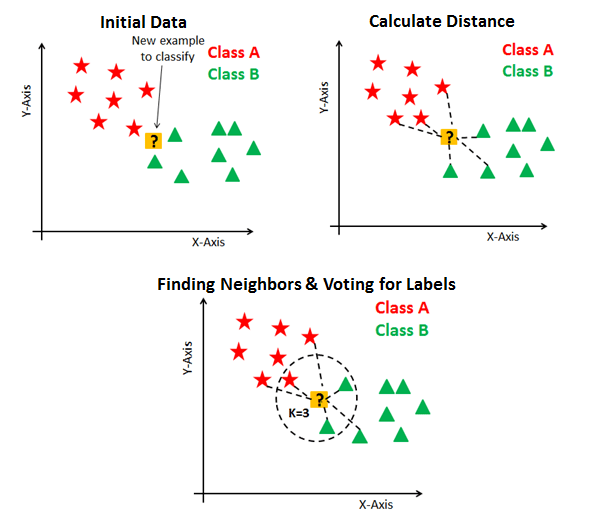
\includegraphics[width = 8cm]{KNN_example.png}
	\end{figure}

		\subsection{Distanza}
			Ovviamente, basandosi sul concetto di vicinanza, bisogna definire la metrica di distanza: la distanza euclidea è una metrica di distanza molto comune, che misura la lunghezza del segmento avente per estremi i due punti.
			$$d(p, q) = \sqrt{(p_{1} - q_{1})^{2} + \dots + (p_{d} - q_{d})^{2}}$$ dove $d$ è la dimensione dello spazio in cui si trovano i punti.
			Per esempio, in uno spazio tridimensionale la formula sarà: $$d(p, q) = \sqrt{(p_{x} - q_{x})^{2} + (p_{y} - q_{y})^{2} + (p_{z} - q_{z})^{2}}$$
			\\[1\baselineskip]
			Bisogna fare attenzione nel caso non si fosse solo interessati a trovare i punti dentro un certo raggio ma si volesse dare più importanza ai punti più vicini a quello preso in questione: un fattore di peso comune è $w = \frac{1}{d^{2}}$.
			\\[1\baselineskip]
			Un altro modo per sensibilizzare la distanza è quello di riscalare i dati. I due metodi più comuni sono:
			\begin{itemize}
				\item $\textbf{StandardScaler}:$ funziona bene se i dati seguono una distribuzione gaussiana/normale. Non rimappa ogni feature nell'intevallo $[0, 1]$ ma dipende dalla variamza: una feature con grande varianza potrebbe impattare fortemente sulla distanza complessiva;
				\item $\textbf{MinMaxScaler}:$ riscala in un range (di default è $[0, 1]$, ma si può modificare). È solitamente più sensibile ai valori anomali, ma pesa le features in maniera più uniforme.
			\end{itemize}

		\subsection{Scelta di K}
			Il valore k nell'algoritmo KNN definisce quanti vicini verranno controllati per determinare la classificazione di un punto specifico.
			Ad esempio, se $k = 1$, l'istanza verrà assegnata alla stessa classe del suo singolo neighbors più vicino.
			\\[2\baselineskip]
			La scelta di $k$ è importante per le performance dell'algoritmo in termini di risultati e di costo computazionale: se $k$ è troppo piccolo l'algoritmo sarà sensibile ai punti di rumore all'interno del dataset, mentre se $k$ è troppo grande il costo di computazione potrebbe crescere di molto.
			\\[1\baselineskip]
			In generale, la scelta di $k$ dipende in gran parte dal dataset poiché i set di dati con più valori anomali probabilmente necessiteranno di valori di $k$ elevati.
			È consigliato di fare tuning del parametro per vedere quale valore porta al risultato migliore e si consiglia di avere un numero dispari per $k$ per evitare pareggi nella classificazione.

		\subsection{Pigrizia e Memoria}
			L'algoritmo KNN fa parte della categoria di algoritmi "lazy", ovvero che il calcolo non viene effettuato durante la sessione di train ma avviene quando viene effettuata una predizione.
			Inoltre fa largo uso della memoria per archiviare i dati di train, il che rende molto costoso in termini di spazio se la dimensionalità dei dati in input è elevata.
\clearpage